\newpage
\section{Fitování a interpolace}
Mějme data reprezentovaná sadou bodů $[(x_i, y_i)]$, kde $x_i$ je řídicí proměnná a $y_i$ je pozorovatelná veličina (např. řídím proud rezistorem a pozoruji napětí). Fit metodou nejmenších čtverců na funkci $f(x; p_1, p_2, ... p_n)$ minimalizuje sumu čtverců reziduí, tj.
\begin{equation}
    R^2 = \sum_i \left|f(x_i, \{p\}) - y_i\right|^2.
\end{equation}
Výsledkem fitu je sada parametrů $\{p\} = p_1, p_2, p_3, ...$, které minimalizují $R^2$. V závislosti na tom, jak funkce $f$ závisí na parametrech $p_k$, mluvíme o \emph{lineárním} nebo \emph{nelineárním} fitování. Důležitý rozdíl je v závislosti na parametrech $p$, nikoli na řídicí proměnné $x$.

% \subsection{Linear Regression}
% TODO

\subsection{Polynomiální fitování}
Fitování polynomem v $x$, kde parametry fitu jsou koeficienty polynomu, je velmi častým příkladem lineárního fitování. Rozhraní pro použití polynomů je obsaženo v podmodulu \ls{np.polynomial} ve třídě \ls{Polynomial}, která poskytuje metodu \ls{fit}. Koeficienty polynomu získáme pomocí metody \ls{Polynomial.convert().coef}. Volání metody \ls{convert()} je nutné, protože \ls{Polynomial} vnitřně mapuje rozsah dat $x$ na interval $[-1, 1]$ (typicky). Příklad použití:

\lstinputlisting[caption=Polynomiální fitování]{../example_code/polynomial_fitting_example.py}
\begin{center}
    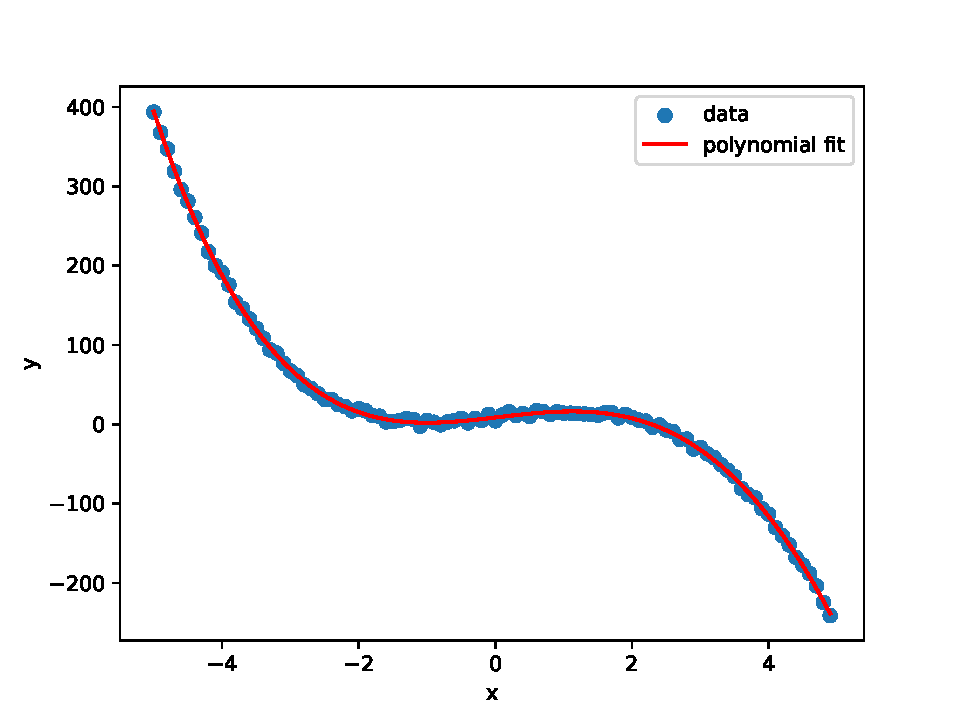
\includegraphics[width=0.5\linewidth]{polynomial_fit.pdf}
\end{center}

\begin{exercise}
    Odečtěte pozadí od píků ve cvičení~\ref{ex:peaks} pomocí polynomiálního fitu.

    \emph{Nápověda}: \ls{np.polynomial.Polynomial.fit()} a booleovská pole
\end{exercise}

\subsection{Nelineární fitování křivek}
Když fitovací funkce závisí nelineárně na parametrech fitu, musíme použít nelineární fitování. Pro tento úkol existuje několik knihoven. Pro základní fitování ale můžeme použít podmodul \ls{scipy.optimize} z \ls{scipy}.

Pro fitování dané funkce na data můžeme použít \ls{scipy.optimize.curve_fit}, např.
\lstinputlisting[caption=Nelineární fitování křivek, label=lst:curve-fit]{../example_code/curve_fit_example.py}
Výstup:
\begin{lstlisting}
    Estimated height: 0.518 +/- 0.007
    Estimated center: 5.039 +/- 0.016
    Estimated width: 2.195 +/- 0.036
\end{lstlisting}
\begin{center}
    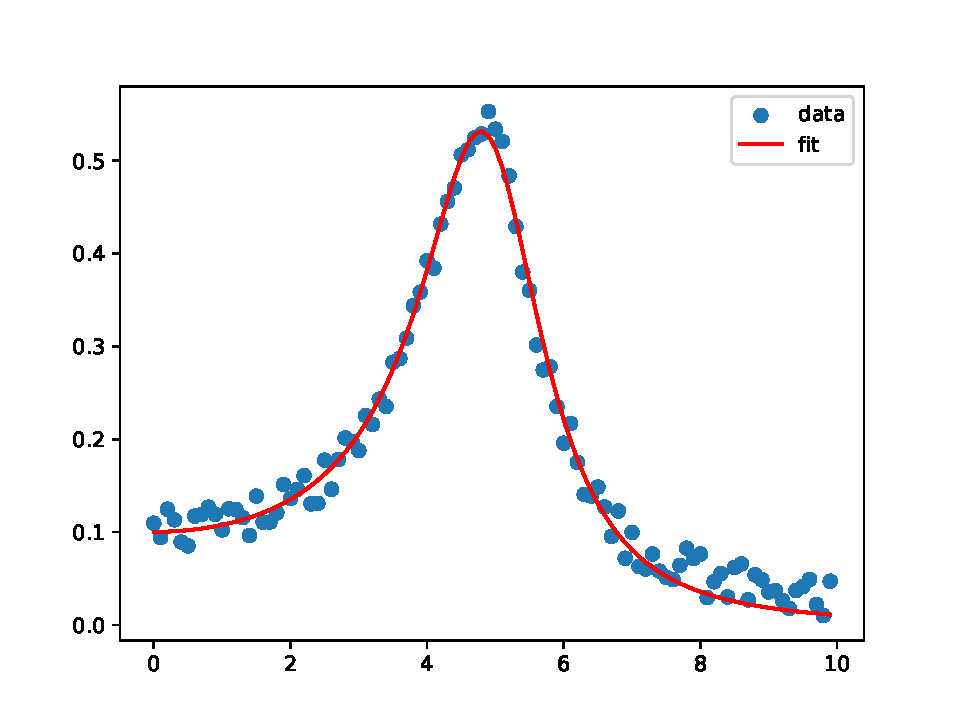
\includegraphics[width=0.5\linewidth]{curve_fit.pdf}
\end{center}

Na rozdíl od lineárních nejmenších čtverců je nelineární fitování křivek iterativní a zastaví se, jakmile parametry skonvergují. U některých kombinací dat a funkce je možné, že fit nemusí nikdy skonvergovat, proto po překročení nakonfigurovaného maximálního počtu iterací fitovací rutiny \emph{vyvolají výjimku} (viz \ref{syn:exceptions}), která shodí program, pokud není ošetřena.

Pro obecnější optimalizační problémy můžeme použít \ls{scipy.optimize.minimize()}. Funkce \ls{minimize()} přijímá jednu \textbf{skalární} funkci (t.j., vracící jedno číslo) a počáteční odhad optimálních parametrů. Například pro nalezení minima dvourozměrné paraboly,
\lstinputlisting[caption=Minimalizace skalární funkce více parametrů]{../example_code/minimize.py}
\begin{center}
    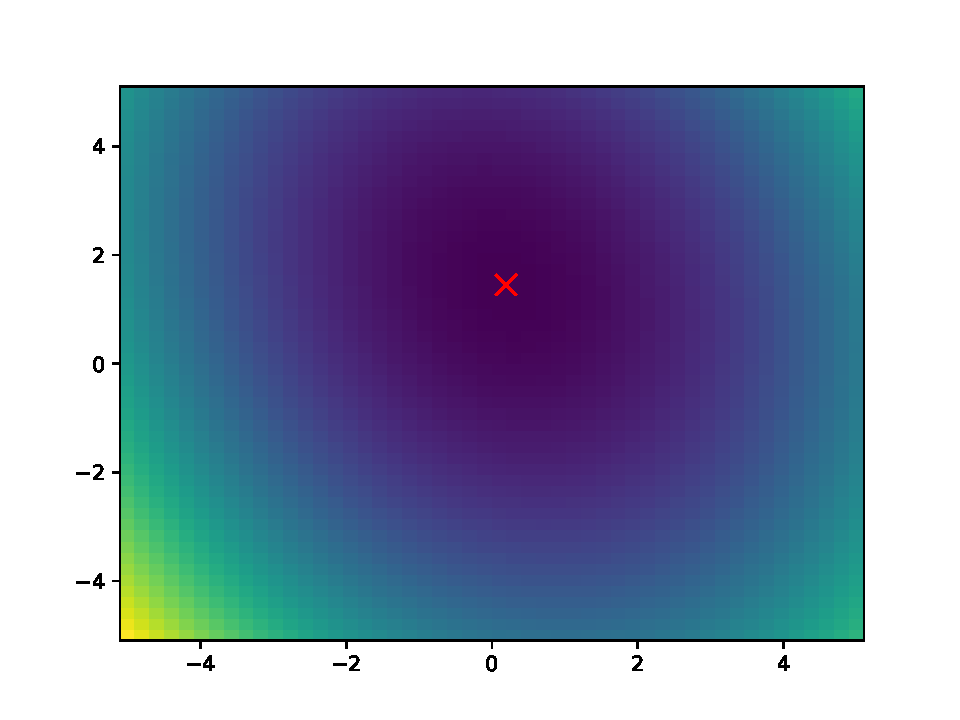
\includegraphics[width=0.5\linewidth]{parabola-minimize.pdf}
\end{center}

\paragraph{Odhad chyby parametrů} Fitovací funkce \ls{curve_fit} vrací dvě hodnoty -- pole parametrů, které nás zajímají, a kovarianční matici parametrů, tj. $\mathrm{cov}(p_i, p_j) = \langle(p_i - \bar p_i)(p_j - \bar p_j)\rangle$. Diagonální hodnoty kovarianční matice lze použít jako odhad nejistot parametrů fitu, tj.
\begin{lstlisting}
    #assuming that f is defined as f(x, p1, p2)
    p, cov = curve_fit(f, x, y)
    print(f"p1 = {p[0]} +/- {np.sqrt(cov[0,0])}")
\end{lstlisting}

Kovarianční matice se počítá z \textit{reziduí} $r_i = y_i - f(x_i, \{p_j\})$, kde $p_j$ jsou optimalizované parametry, jako ($\mathbf{r}$ je vektor s prvky $r_i$; $i=1\dots N$, $j=1\dots M$; $N$ je počet datových bodů a $M$ je počet parametrů) škálovaná inverze Hessovy matice $H$ optimalizované funkce $\chi^2 = \sum r_i^2$\footnote{Výpočet je mírně složitější, ale podobný, když mají datové body různé váhy, viz \href{https://docs.scipy.org/doc/scipy/reference/generated/scipy.optimize.curve_fit.html}{dokumentace}}
\begin{equation}
    \mathrm{cov}(p_i, p_j) = \frac{1}{N-M}
    \begin{pmatrix}
        \frac{\partial \chi^2}{\partial p_1 \partial p_1} & \frac{\partial \chi^2}{\partial p_1 \partial p_2} & \dots \\
        \frac{\partial \chi^2}{\partial p_1 \partial p_1} & \frac{\partial \chi^2}{\partial p_2 \partial p_2} & \dots\\
        \vdots & \vdots & \ddots
    \end{pmatrix}^{-1},
\end{equation}
Obvykle nás zajímá pouze diagonála pro přímý odhad chyby parametrů fitu, všimněte si, však ale, že pokud je například studovaná veličina součtem dvou parametrů fitu $z = A + B$, pak rozptyl $z$ je
\begin{equation}
    \mathrm{var} z = \langle (A + B - \bar A - \bar B)^2 \rangle = \langle (A - \bar A)^2 \rangle + \langle (B - \bar B)^2 \rangle + 2\langle (A - \bar A) (B - \bar B) \rangle = \mathrm{var} A + \mathrm{var} B + 2\mathrm{cov}(A, B),
\end{equation}
a musí být použity i mimodiagonální členy kovarianční matice.

Odhad chyb vypočtený pomocí kovarianční matice však může být často podhodnocen, protože výše uvedená metoda je platná pouze tehdy, když je modelová funkce $f$ správná a data mají skutečně tvar $y_i = f(x_i, p) + e_i$, kde chyby dat $e_i$ mají nulovou střední hodnotu a normální rozdělení. Robustnější, ale také výpočetně náročnější metodou odhadu chyb parametrů je \textbf{bootstrap}, kde pro několik opakování vytvoříme náhodný výběr dat (stejné délky), provedeme fit na každé vytvořené sadě a vypočítáme průměr a směrodatnou odchylku (a v principu i kovarianci) na výsledné sadě parametrů fitu. Příklad implementace je ukázán v Lst.~\ref{lst:bootstrap}.

\lstinputlisting[firstline=24, caption=Odhad chyb parametrů fitu pomocí bootstrapu. Data 
%$(x_i, y_i)$
 jsou vytvořena stejným způsobem jako v Lst.~\ref{lst:curve-fit}., label=lst:bootstrap]{../example_code/bootstrap_curve_fit_example.py}

\begin{syntax}[Výjimky a ošetřování chyb]
    \label{syn:exceptions}
    Výjimky jsou mechanismus, který Python používá k signalizaci chyb nebo jiných událostí, které musí váš kód ošetřit. Pokud \emph{vyvolaná} výjimka není \emph{zachycena}, program spadne. K ošetření výjimek používáme bloky \ls{try}, \ls{except} a \ls{finally}. Výjimku můžeme vyvolat pomocí \ls{raise}. Všimněte si, že výjimky nemusí vždy znamenat chybu, například cyklus \ls{for} je ukončen pomocí výjimky \ls{StopIteration}.

    Příklad zachycení a vyvolání výjimek a použití bloku \ls{finally}.
\begin{lstlisting}
def faulty_function():
    raise ValueError("blergh!")

xs = [-2, -1, 0, 1, 2]
one_over_xs = []
try:
    for x in xs:
        try:
            one_over_xs.append(1/x)
            if x > 1:
                faulty_function()
        except ZeroDivisionError:
            print("Can't divide by zero!")
        except:
            print("something else went wrong")
            raise #propagate the exception further up
finally:
    print("I will always run")

# unless the exception that is raised on line 9 and then sent forward
# on line 16 isn't  handled, this line will not run
print(one_over_xs)
\end{lstlisting}
    Všimněte si několika věcí:
    
    \textbf{\ls{except}} Může zachytit buď specifický typ výjimky, nebo jakýkoli typ (pokud typ výjimky není specifikován).
    
    \textbf{Blok \ls{finally} se vždy spustí}, bez ohledu na to, zda uvnitř bloku \ls{try} došlo k výjimce, a je obecně určen pro řádné uvolnění zdrojů (např. otevřených souborů).
        
    \textbf{Bloky \ls{try} mohou být vnořené}: Když je vyvolána výjimka, nejvnitřnější blok \ls{try-except} se ji pokusí ošetřit. Pokud není nalezen vhodný \ls{except} nebo je výjimka znovu \ls{raise}-nuta, pokusí se ji ošetřit další obklopující blok \ls{try-except} a tak dále. Pokud se výjimka dostane ze všech vnořených obklopujících bloků \ls{try-except} bez ošetření, program spadne.
    
    \textbf{\ls{raise} lze použít kdekoli}, např. ve funkcích, které neobsahují \ls{try}. Je na volajícím kódu, aby rozhodl, co s výjimkami udělá.
\end{syntax}

\begin{exercise}
    \label{ex:peak-fits}
    Fitujte absolutní hodnotu $r(f) = \sqrt{x^2 + y^2}$ odezvy ve cvičení~\ref{ex:peaks} na odezvu lineárního harmonického oscilátoru plus polynomiální pozadí (stupeň polynomu 3) a vykreslete výsledky podobně jako ve cvičení~\ref{ex:peaks}. Použijte jednoduchý odhad ze cvičení~\ref{ex:peak} jako počáteční odhady parametrů fitu. Použijte řešení cvičení~\ref{ex:peak} jako modul.

    Bonusové cvičení: udělejte stupeň polynomu pozadí nastavitelný.

    Komplexní amplituda odezvy lineárního harmonického oscilátoru na sílu $F$ je (viz Dodatek~\ref{sec:lho})
    \begin{equation}
        x(\omega) = \frac{F/m}{\omega_0^2 - \omega^2 + i\omega\gamma},
    \end{equation}
    kde $\omega_0$ je (úhlová) rezonanční frekvence, $\omega$ je frekvence síly $F$, $m$ je hmotnost oscilátoru a $\gamma$ je tlumení.
\end{exercise}
\begin{exercise}
    Odhadněte chyby parametrů fitu získaných ve cvičení~\ref{ex:peak-fits} pomocí bootstrapu.
\end{exercise}

% TODO: lmfit

